%% LyX 2.2.3 created this file.  For more info, see http://www.lyx.org/.
%% Do not edit unless you really know what you are doing.
\documentclass[english]{article}
\usepackage[T1]{fontenc}
\usepackage[latin9]{inputenc}
\usepackage{geometry}
\geometry{verbose,tmargin=2cm,bmargin=2cm,lmargin=2cm,rmargin=2cm,headheight=2cm,headsep=2cm}
\setlength{\parindent}{0bp}
\usepackage{float}
\usepackage{graphicx}

\makeatletter
%%%%%%%%%%%%%%%%%%%%%%%%%%%%%% User specified LaTeX commands.
\usepackage{babel}

\makeatother

\usepackage{babel}
\begin{document}

\title{Final Practical Work Electronics III}

\author{M�ller, Malena\\
 Diaz, Ian Cruz\\
 Oh, Victor\\
 Lin, Benjamin}
\maketitle

\section{Summary}

In this work we were asked to implement a precise chronometer, digital
electronics, and a VGA screen of 640 pixels wide and 480 pixels in
height. We were provided with a Cyclone IV Field Programmable Gate
Array, also known as FPGA, and we had to create the inside digital
logic using Verilog Hardware Descriptive Language. The implementation
of this chronometer is explained in detail in the following sections.

\section{How VGA Works}

The functioning of the VGA protocol is very simple, as shown in Figure
\ref{1}, we only have to analyze 5 of its pins. Whatever the V\_SYNC
pin receives, corresponds to the vertical synchronization of the screen,
while the H\_SYNC pin receives what corresponds to its horizontal
synchronization. The R, G and B wires correspond to the Red, Geen
and Blue colors of the pixel to print. So, if we call $T_{H}$ to
the h\_sync period and $T_{V}$ to the v\_sync period, to reference
a single pixel as line-column, the formulas are the following:

\begin{equation}
Line=\frac{T_{V}}{480}*(time\,h_{sync}\,is\,on)\label{eq:1}
\end{equation}

\begin{equation}
Column=\frac{T_{H}}{640}*(time\,v_{sync}\,is\,on)\label{eq:2}
\end{equation}

\begin{figure}[H]
\begin{centering}
\includegraphics[scale=0.5]{\string"Images/VGA pins\string".eps} 
\par\end{centering}
\caption{VGA Pins}
\label{1}
\end{figure}

\section{Implementation}

To implement the chronometer, we follow the diagram shown on Figure
\ref{2}, we used a h\_sync and v\_sync generator module, a Screen
Positioning Module, a Time Counter Module, a Timer Module and a binary
to a 7 segments display module.

\begin{figure}[H]
\begin{centering}
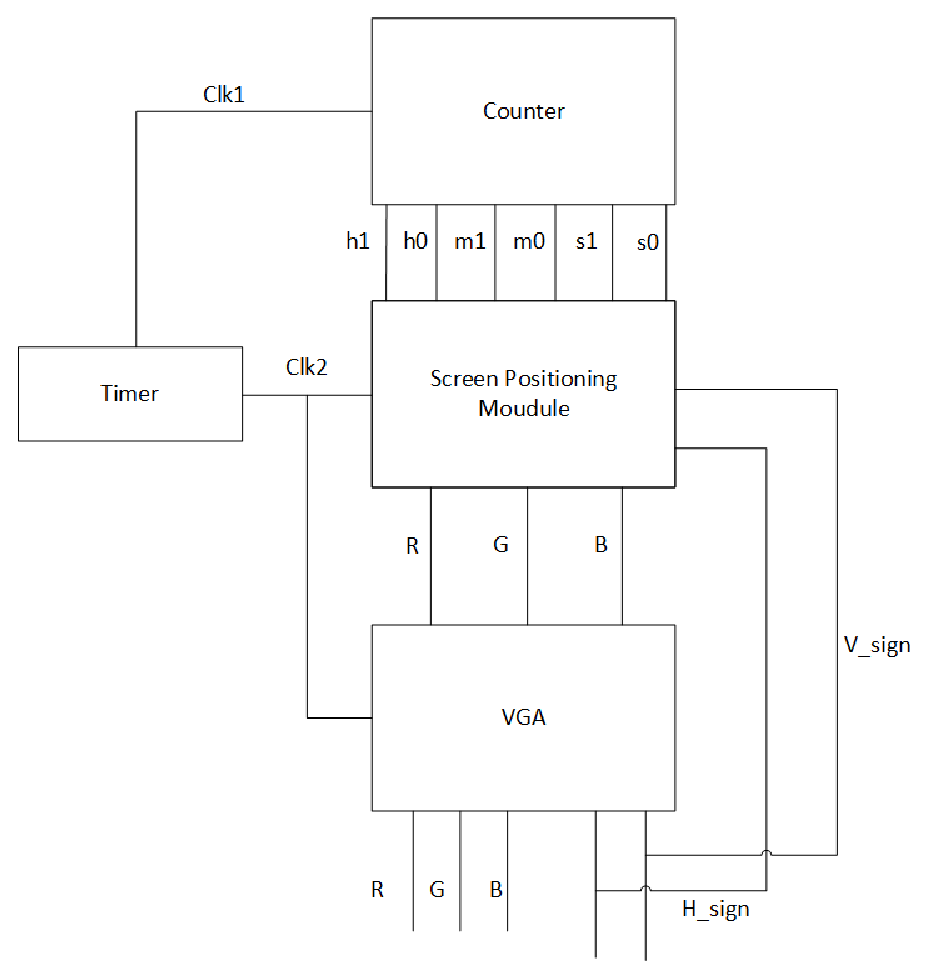
\includegraphics[scale=0.4]{Images/Modulos}
\par\end{centering}
\caption{Implementation Diagram}
\label{2}
\end{figure}

\subsection{VGA Module}

This module corresponds to the Video Graphics Array (VGA), which is
a graphics standard for video display. There are five pins in the
VGA connector, that we have to control: the V\_SYNC, H\_SYNC, R, G
and B, shown in Figure \ref{1}. We needed to send five signals, one
to each of these five different monitor's pins. This signals' generator
module was made in Verilog. It outputs the following signals:
\begin{description}
\item [{-Vsync:}] The vertical synchronization's signal.
\item [{-Hsync:}] The horizontal synchronization's signal.
\item [{-R:}] The signal corresponding to the red component of a pixel.
\item [{-G:}] The signal corresponding to the green component of a pixel.
\item [{-B:}] The signal corresponding to the blue component of a pixel.
\end{description}
We used a resolution of 640x480. The Vsync signal is responsible of
updating the entire display, in each of its periods. In order to do
so, the Hsync signal updates one horizontal line of the display in
each of the Hsync signal's period. The R, G and B signals update the
color of one pixel.

The vertical sync is formed by four parts, in the following order:
vertical sync pulse, vertical back porch, vertical display and vertical
vertical front porch. As well as the vertical sync signal, the horizontal
sync is formed by a horizontal sync pulse, horizontal back porch,
horizontal display and horizontal front porch. These signals are 1
only during their sync pulses. For the rest of the parts that form
these signals, their value is 0. Moreover, the display colors are
only shown during the vertical display time and horizontal display
time of these signals. This means that while both the Vsync and Hsync
signals are in their display part of the period, the R, G and B signals
output the values corresponding to the pixel that has to be shown
in that position of the screen. For the rest of the time, the R, G
and B signals are 0.

Four Verilog modules were made to generate these signals. The Vsync
module, Hsync module, RGB module, and finally the VGA module which
includes the previously mentioned three modules.

\subsubsection{Vsync Module}

This module generates and it outputs the entire Vsync signal, and
it also outputs a vertical display sigal which is in 0 only when colors
can appear in the corresponding vertical position.

\subsubsection{Hsync Module}

This module generates and it outputs the entire Hsync signal, and
it also outputs a horizontal display signal which is in 0 when colors
can appear in the corresponding horizontal position.

The vertical display and the horizontal display signals are not sent
to the VGA pins, but they are used by the Screen Positioning Module,
in order to know when to update the pixels' colors.

\begin{figure}[H]
\begin{centering}
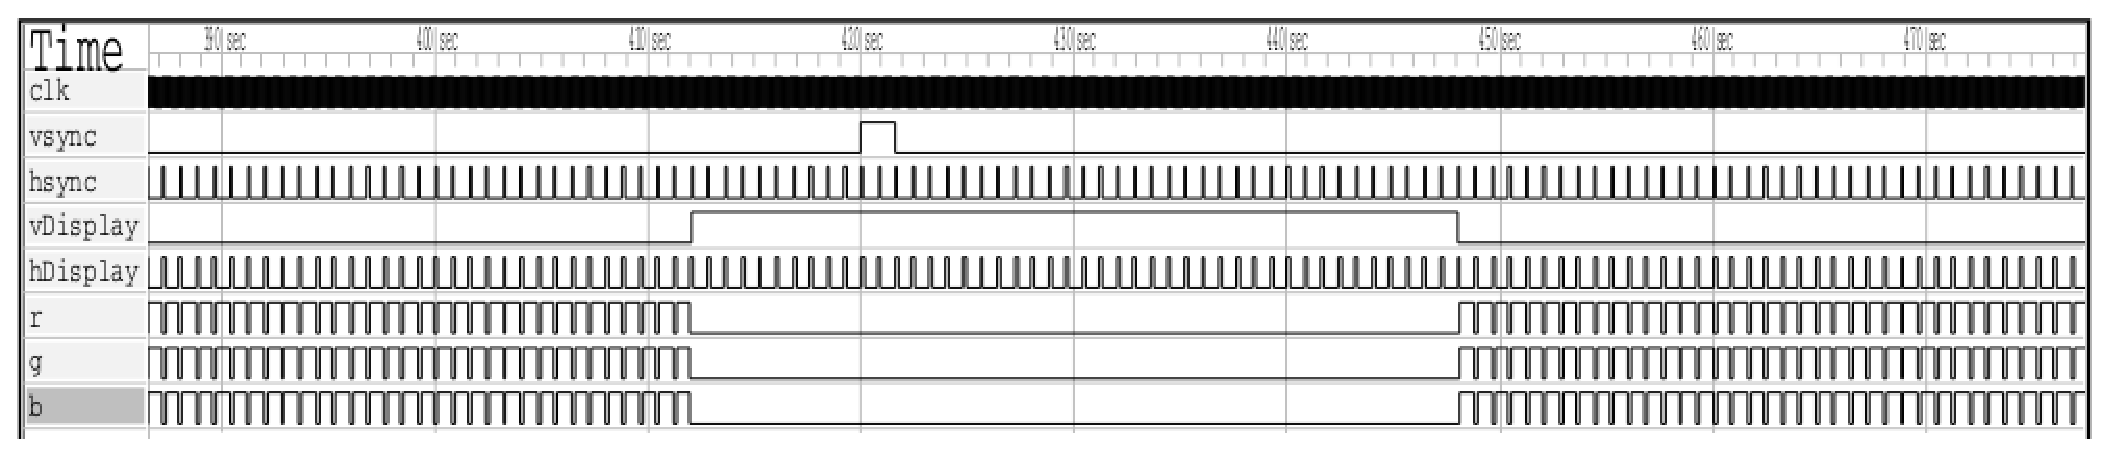
\includegraphics[scale=0.3]{Images/Sim1}\\
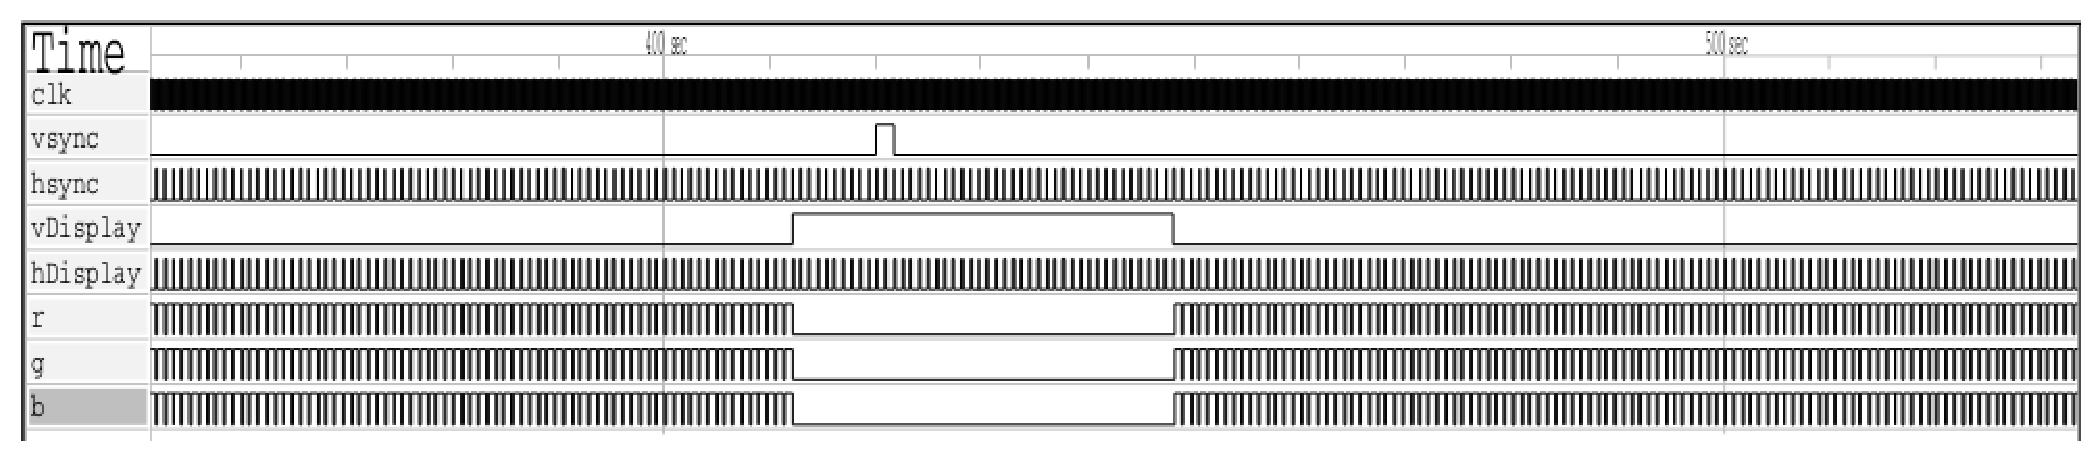
\includegraphics[scale=0.3]{Images/Sim2}\\
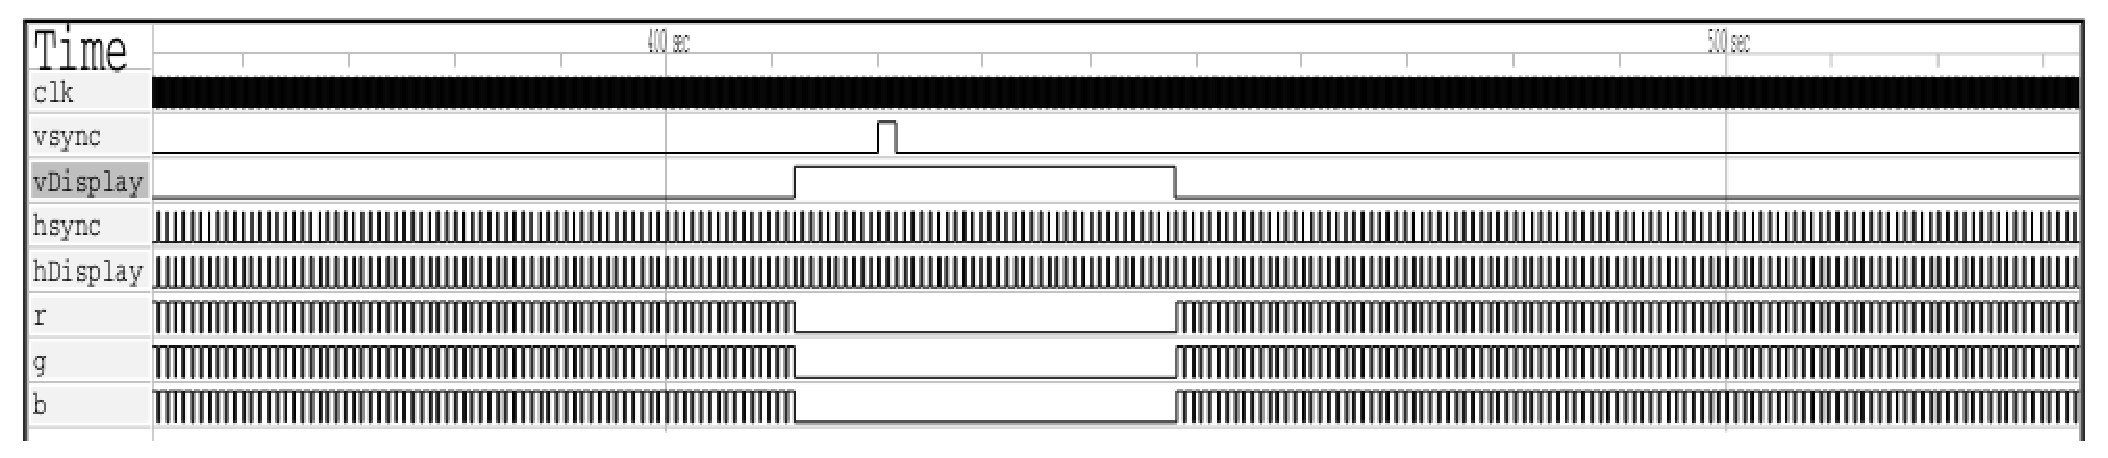
\includegraphics[scale=0.3]{Images/Sim3}\\
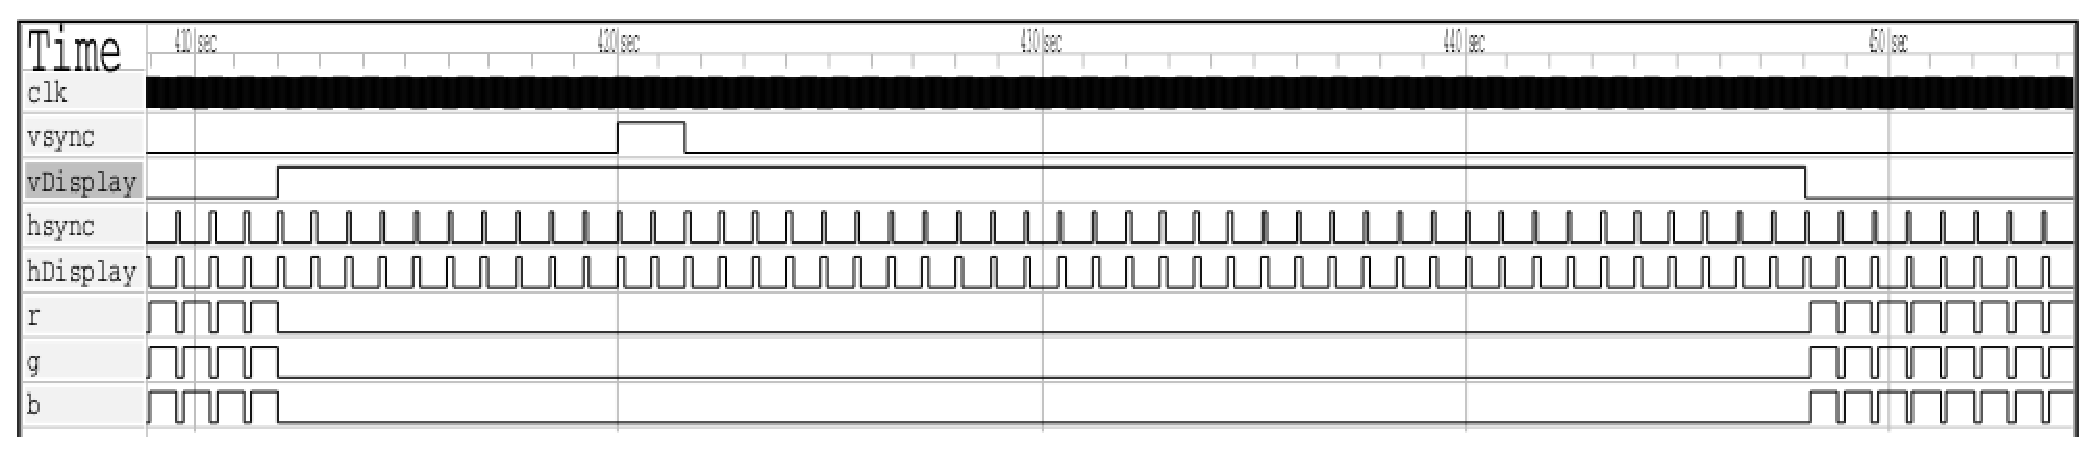
\includegraphics[scale=0.3]{Images/Sim4}\\
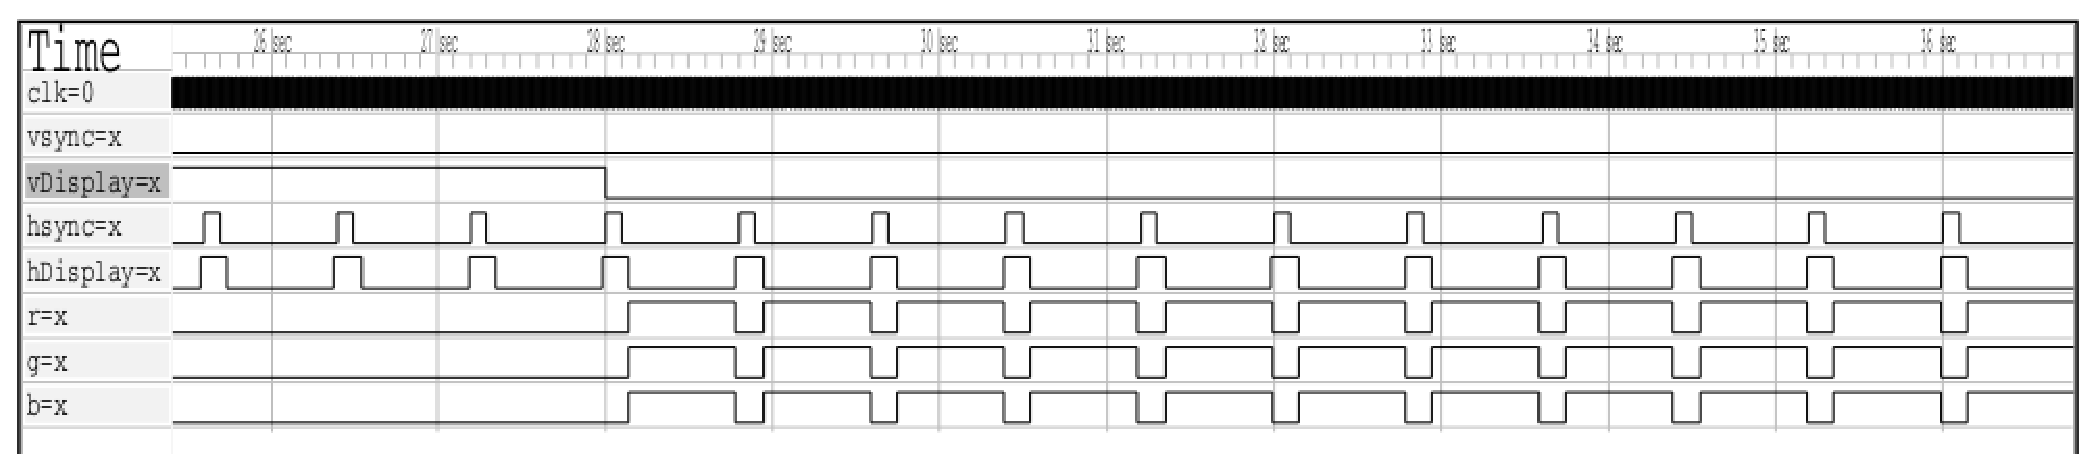
\includegraphics[scale=0.3]{Images/Sim5}
\par\end{centering}
\caption{GTK Wave SImulations}
\label{4}

\end{figure}

In Figure \ref{4} we can see the functioning of the previously mentioned
signals. The vertical display and the horizontal display signals are
not sent to the VGA pins, but they are used by the Screen Positioning
Module, in order to know when to update the pixels' colors.

\subsubsection{RGB Module}

This module generates the R, G and B output signals.

\subsection{Screen Positioning Module}

For this module, we received the same signals sent to the VGA (h\_sync
and v\_sync), the BCD digits of the hours, minutes and seconds counted,
and a clock working at the same speed as the h\_sync clock for each
pixel. The outputs of this module, were connected to the H\_sync and
V\_sync Generato Module, and this are the R , G and B colors of the
VGA pixels.

\subsubsection{Operation}

The operation of this module is pretty straight foward, by knowing
the h\_sync and the v\_sync signals, and having the same clock as
the h\_sync generator, it determines at each moment in wich pixel
it is working on. To do this, it utilizes the equations (\ref{eq:1})
and (\ref{eq:2}), and by knowing the position, it devides the screen
in quadrants for each digit of the chronometer. Whenever it detects
that it is on a digit quadrant, it uses the NumTo7Seg module to convert
the correspond digit to a series of 7 bits, as if it where a 7 segment
display, and by knowing each pixel, it determines which pixel it has
to print in white, and which in black.

Finally, it feedbacks the H-sync and V\_sync Generator module with
the colors processed in this module. A simulation of this module was
made in GTK wave before uploading to the FPGA, and as we see on Figure
\ref{3}, we can conclude that it behaves as expected to.

\begin{figure}[H]
\noindent \begin{centering}
\includegraphics[scale=0.4]{\string"Images/Simulacion 1\string".eps}
\par\end{centering}
\noindent \begin{centering}
\includegraphics[scale=0.4]{\string"Images/Simulacion 2\string".eps}
\par\end{centering}
\caption{Simulation GTK Wave}
\label{3}
\end{figure}

\subsection{Time Counter Module}

To measure times down to the millisecond, a counter module was employed.

\subsubsection{Design:}

Since the counter is designed to count time units, a clock input was
needed. Also, since the main functions on a stopwatch are START/STOP
and RESET, the \textquotedbl{} Enable\textquotedbl{} and \textquotedbl{}
Reset\textquotedbl{} inputs were also taken into account in the design.
Finally, to properly communicate with the modules for displaying the
time, the module was designed to output each digit in BCD format.

Given that the format chosen was HH:mm:ss, 6 BCD output in total were
required. In addition, for future implementation, the millisecond
digits were also taken into account.

Since the tasks at hand were to: 
\begin{itemize}
\item Count the number of milliseconds passed 
\item Calculate the corresponding number of hours, minutes and seconds passed 
\item Convert each quantity to BCD numbers 
\item Scale down the clock frequency 
\end{itemize}
The module was designed with 3 sub-modules: a \textquotedbl{} counter\textquotedbl{}
module, a \textquotedbl{} watch format\textquotedbl{} module, a \textquotedbl{}
binary to BCD\textquotedbl{} module and a \textquotedbl{} frequency
divider\textquotedbl{} module.

\subsubsection{How it works:}

First, the frequency divider module converts the FPGA's 50 MHz to
the required 1 kHz for the counter module to actually count milliseconds.
Second, the counter module, as per the name, counts the number of
milliseconds that pass. Since this count needs to reach 100 hours
maximum, the size of this counter is 29 bits. Third, the \textquotedbl{}
watch format\textquotedbl{} module converts the number of millisecons
to its respective units: ms to hr, ms to min, and ms to s, taking
into account the format in which the data will be presented. Finally,
to send this data to the display modules, each quantity is converted
into its respective BCD digits. For example, if the \textquotedbl{}
watch format\textquotedbl{} module returns 59s, the \textquotedbl{}
binary to BCD\textquotedbl{} module will convert it into a 5 and a
9, each in BCD format.

The RESET and ENABLE inputs only interact with the counter module.
The RESET signal will clear the counter and set it back to 0. The
ENABLE signal activates or deactivates the counter. In other words,
if it is low, the count will not increase.
\end{document}
